\documentclass[12pt]{report} 

% PACKAGES 
\usepackage[dutch]{babel}
\usepackage[utf8]{inputenc}
\usepackage{color}
\usepackage{amsmath} % Matrices
\usepackage{amsfonts}
\usepackage{enumitem}
\usepackage{booktabs}
\usepackage{xcolor}
\usepackage{sectsty}
\usepackage{graphicx}
\usepackage{lipsum}

\graphicspath{{img/}}

\newcommand{\answercolor}{teal}


\partfont{\color{brown}}
\chapterfont{\color{teal}}
\sectionfont{\color{cyan}}

% DOCUMENT INFORMATION
\title{Wiskunde A}
\author{Bert De Saffel}
\date{2017-2018}


% CUSTOM COMMANDS
\newcommand{\todo}[1] {
\color{red}\textunderscore{\textit{TODO: #1}}
}

\newcommand{\important}[1] {\textbf{\color{orange}#1}}
\newcommand{\mathimportant}[2] {\textbf{\color{#2}$#1$}}

% DOCUMENT
\begin{document}
\maketitle
\tableofcontents

\part{Theorie}
\chapter{Complexe Getallen}
\important{Inleiding}
\begin{itemize}
 \item $\mathbb{N}$ = Natuurlijke getallen: \{0, 1, 2, 3, ...\}
 \item $\mathbb{Z}$ = Gehele getallen: \{..., -2, -1, 0, 1, 2, ...\}
 \item $\mathbb{Q}$ = Rationale getallen: \{$\frac{1}{3}$, $-\frac{1}{4}$, $\frac{7}{2}$, ... \}
 \item $\mathbb{R}$ = Reële getallen: \{ $\sqrt{2}$ , $\pi$ \}
 \item $\mathbb{C}$ = Complexe getallen: $j^2 = -1$, $j = $ imaginaire eenheid
\end{itemize}
\important{Definitie}
$z = \mathimportant{a}{orange} + \mathimportant{b}{orange}j$ met $z \in \mathbb{C}$, $a \in \mathbb{R}, b \in \mathbb{R}$ en $j = \sqrt{-1}$ met
\begin{itemize}
 \item $Re(z) = a$
 \item $Im(z) = b$
\end{itemize}
\important{3 Vormen}
\begin{itemize}
 \item Cartesische vorm: $z = a + bj$
 \item Goniometrische vorm: $z = r[cos(\theta) + jsin(\theta)]$
 \item Exponentiële vorm: $re^{j\theta}$
\end{itemize}
\important{Vlak van Gauss}
\begin{itemize}[label={}]
 \item 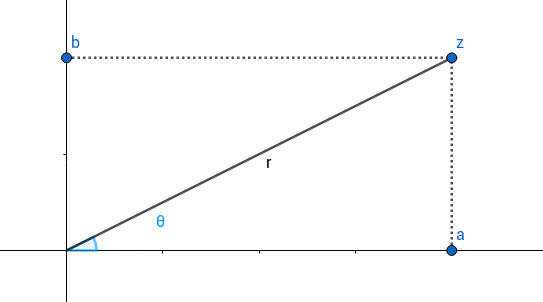
\includegraphics[width=\linewidth]{goniometrischevorm}
\end{itemize}
\important{a en b}
\begin{itemize}
 \item $a = rcos(\theta)$
 \item $b = rsin(\theta)$
\end{itemize}
\important{r en $\theta$}
\begin{itemize}
 \item $r \geq 0$
 \item $r = \sqrt{a^2 + b^2}$
 
 \item $\theta \in [0, 2\pi]$
 \item $\theta \in ]-\pi, \pi[$
 \item $tg(\theta) = \frac{b}{a} (+ \pi)$
\end{itemize}
\important{Complex toegevoegde}
\begin{itemize}
 \item Cartesische vorm: $\overline{z} = a - bj$ 
 \item Exponentiële vorm: $\overline{z} = re^{-j\theta}$
\end{itemize}
\important{Bewerkingen}
\begin{itemize}
 \item $z_1 + z_2$
 \item $z_1 . z_2 = (r_1 . r_2)e^{j(\theta_1 + \theta_2)}$
 \item $\frac{z_1}{z_2} = \frac{r_1}{r_2}e^{j(\theta_1 - \theta_2)}$
 \item $z^{n} = r^{n}e^{jn\theta}$
 \item $\sqrt[n]{z} = r^{\frac{1}{n}}e^{j\frac{1}{n}}(\theta + 2k\pi)$
\end{itemize}

\chapter{Limieten}
\important{Limiet naderen}
\begin{itemize}
 \item $\lim_{x\to\infty} f(x) = \lim_{x\to-\infty} en \lim_{x\to+\infty}$
 \item $\lim_{x\to a} f(x) = \lim_{x\to a^-} en \lim_{x\to a^+}$ met $a \in \mathbb{R}$
\end{itemize}
\important{Bijzondere limieten}
\begin{itemize}
 \item $\lim_{x\to\infty} 
 \frac{a_nx^n + a_{n - 1}x^{n - 1} + ... + a_1x + a_0}{b_kx^k + b_{k - 1}x^{k - 1} + ... + b_1x + b_0}
 = \frac{a_nx^n}{b_kx^k}$
 \item $\lim_{x\to0} \frac{sin(x)}{x} = 1$
 \item $\lim_{x\to0} \frac{tg(x)}{x} = 1$
 \item $\lim_{x\to\infty} (1 + x)^{\frac{1}{x}} = \lim_{y\to\infty}(1 + \frac{1}{y})^y = e$
\end{itemize}
\important{Onbepaaldheden}
\begin{itemize}
 \item $\frac{0}{0}$
 \item $\frac{\infty}{\infty}$
 \item $+ \infty - \infty$
 \item $0 . \infty$
 \item $0^0$
 \item $\infty^0$
 \item $1^\infty$
\end{itemize}
\important{Wegwerken onbepaaldheden}
\begin{itemize}
 \item Gemeenschappelijke factor van teller en noemer vinden
 \item Toegevoegde waarde van teller, noemer of beiden
 \item $f(x) * g(x) = \frac{f(x)}{1/g(x)}$
 \item $f(x)^{g(x)} = e^{ln(f(x)^{g(x)})}$
 \begin{enumerate}[label={}]
     \item Geldig voor:
     \item $0^0$
     \item $\infty^0$
  \end{enumerate}
 \item $\lim_{x\to...} (1 + g(x))^{\frac{1}{g(x)}}$
  \begin{enumerate}[label={}]
       \item Geldig voor:
    \item $1^\infty$
  \end{enumerate}

\end{itemize}



\part{Oefeningen}
\chapter{Complexe Getallen}
  \begin{itemize}
   \item $1)z_1$
   \begin{itemize}
     \item \important{Cartesische vorm} : $z_1 = -1 + \sqrt{3}j$
     \item \begin{enumerate}
            \item Bereken: $r = \sqrt{-1^2 + \sqrt{3}^2}$
			    = $\sqrt{1 + 3} = \sqrt{4} = 2$
	    \item Bereken: $\theta = bgtg(\frac{\sqrt{3}}{-1})$
			    = $bgtg(-\sqrt{3}) = -\frac{\pi}{3} + \mathimportant{\pi}{orange}$
			    \newline
			    $+\pi$ aangezien $(-1, \sqrt{3} =$ 
			    kwadrant \textup{\uppercase\expandafter{\romannumeral2}})
			    = $\frac{2\pi}{3}$
           \end{enumerate}
     \item \important{Goniometrische vorm} : $z_1 = 2[cos(\frac{2\pi}{3}) + jsin(\frac{2\pi}{3})]$
     \item \important{Exponentiële vorm} : $z_1 = 2e^{j\frac{2\pi}{3}}$

    \end{itemize}
   \item $4)z_1 = - 1 + j\;\;\;z_2 = e^{-\frac{\pi}{4}j}$
   \begin{itemize}
    \item $z = z_1.\overline{z_2}$
     \begin{enumerate}
           \item $z_1$ Vorm om naar exponentiële vorm: $z_1 = \sqrt{2}e^{j\frac{3\pi}{4}}$
           \item $z_1 . \overline{z_2}$: $\sqrt{2}e^{j\frac{3\pi}{4}}\;.\;e^{j\frac{\pi}{4}}$
            = $(\sqrt{2} . 1)e^{j(\frac{3\pi}{4} + \frac{\pi}{4})}$ = $\mathimportant{\sqrt{2}e^{j\pi}}{orange}$
          \end{enumerate}
    \item $z = \frac{z_1}{j} . z^{3}_2$
      \begin{enumerate}
       \item Bereken $\frac{z_1}{j}$ = $\frac{-1 + j}{j} . \mathimportant{\frac{-j}{-j}}{red}$ = $\frac{-j(-1 + j)}{j(-j)}$
	= $\frac{-j(-1 + j)}{-j^2}$ = $\frac{j + 1}{1}$ = $1 + j$
	\item Vorm om naar exponentiële vorm: $\sqrt{2}e^{j\frac{\pi}{4}}$
	\item Bereken $z^{3}_2$ = $(e^{-\frac{\pi}{4}j})^3$ = $e^{-\frac{3\pi}{4}j}$
	\item Vermenigvuldig: $\sqrt{2}e^{j\frac{\pi}{4}}\;.\;e^{-\frac{3\pi}{4}j}$
	= $\mathimportant{\sqrt{2}e^{-\frac{\pi}{2}j}}{orange}$

     \end{enumerate}

   \end{itemize}

   \item $2)z = (\frac{1}{3} - \frac{\sqrt{3}}{3}j)^5$
   \begin{enumerate}
    \item Vorm $\frac{1}{3} - \frac{\sqrt{3}}{3}j$ om naar exponentiële vorm = $\frac{2}{3}e^{-\frac{\pi}{3}j}$
    \item Bereken: $(\frac{2}{3}e^{-\frac{\pi}{3}j})^5$ = $\frac{2^5}{3^5}e^{-\frac{5\pi}{3}j}$ = $\frac{2^5}{3^5}e^{\frac{\pi}{3}j}$
    \item Bereken: $a = \frac{2^5}{3^5}cos(\frac{\pi}{3})$ = $\frac{2^5}{3^5} . \frac{1}{2} = \frac{2^4}{3^5} = \frac{16}{243}$
    \item Bereken: $b = \frac{2^5}{3^5}sin(\frac{\pi}{3})$ = $\frac{2^5}{3^5} . \frac{\sqrt{3}}{2} = \frac{16\sqrt{3}}{243}$
    \item $z = \frac{16}{243} + \frac{16\sqrt{3}}{243}j$
  \end{enumerate}


  \end{itemize}

  
\end{document}
